% Total economic value decomposition
\documentclass[tikz,border=4pt]{standalone}
\renewcommand\familydefault{\sfdefault}
\usetikzlibrary{shapes.arrows,positioning}
\begin{document}
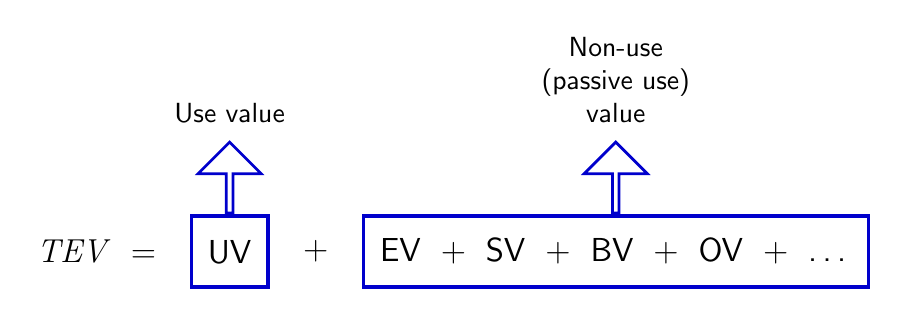
\begin{tikzpicture}[
    box/.style={draw=blue!80!black, line width=1.2pt, inner sep=6pt, minimum height=9mm, font=\large},
    up/.style={single arrow, draw=blue!80!black, line width=1pt, fill=white,
               shape border rotate=90, minimum height=9mm, minimum width=8mm,
               single arrow head extend=1.5mm, inner sep=0pt},
    lbl/.style={align=center}
  ]
  \node[font=\large] (tev) {$\mathit{TEV}\;=$};
  \node[box, right=3mm of tev] (uv) {UV};
  \node[font=\large, right=3mm of uv] (plus) {$+$};
  \node[box, right=3mm of plus] (nuv) {EV \;+\; SV \;+\; BV \;+\; OV \;+\; \dots};
  \node[up, above=0pt of uv.north]  (a1) {};
  \node[up, above=0pt of nuv.north] (a2) {};
  \node[lbl, above=1mm of a1] {Use value};
  \node[lbl, above=1mm of a2] {Non-use\\(passive use)\\value};
\end{tikzpicture}
\end{document}
